
    \chapter{Introdução}

    Desde os tempos antigos os m\'{e}todos de pagamento e manipulação de dinheiro vêm mudando de maneira constante. Segundo \citeonline{tellez2017}, antes de haver um sistema monetário o pagamento era feito com trocas de mercadoria e isso foi eficiente enquanto as necessidades humanas eram limitadas. Entretanto, com o crescimento da complexidade da sociedade, este método se tornou insuficiente e o homem teve que adotar outros sistemas como moedas de minério, e após isso, dinheiro e o cart\~{a}o banc\'{a}rio. Com o avanço tecnológico, rápido desenvolvimento da tecnologia de redes móveis e os avanços nos dispositivos portáteis, tornou-se possível que as pessoas acessassem a Internet usando dispositivos móveis em qualquer lugar e a qualquer hora para realizar transações de comércio eletrônico e outras operações, como navegação na web, leitura de e-mail e assim por diante. Dessa forma, foi possível a criação de novos m\'{e}todos pr\'{a}ticos, fáceis e r\'{a}pidos de pagamento e manipulação de dinheiro.
    
    
    O banco móvel, segundo \citeonline{Singhal2019}, se refere à provisão de serviços bancários, tais como transferências, verificação de saldos, efetuação de pagamentos, investimentos e outras transações, através de dispositivos portáteis que suportam aplicativos - smartphones, tablets e, em alguns casos, smartwatches. Com essa capacidade, os clientes têm à disposição a maioria dos serviços oferecidos por suas instituições financeiras na palma de suas mãos, sem a necessidade de visitar uma agência bancária ou um caixa eletrônico, nem de estar em frente a um computador de mesa ou laptop. 
    
    As estatísticas \cite{Deloitte2021} confirmam que a adoção dessa abordagem de interação com as instituições financeiras está ganhando força. Na figura \ref{MobileBanking} pode-se observar alguns exemplos de bancos que fornecem aplicações bancárias, como Banco do Brasil, Bradesco, Caixa, Itaú e Santander.

    \begin{figure}[H]
    \centering 
    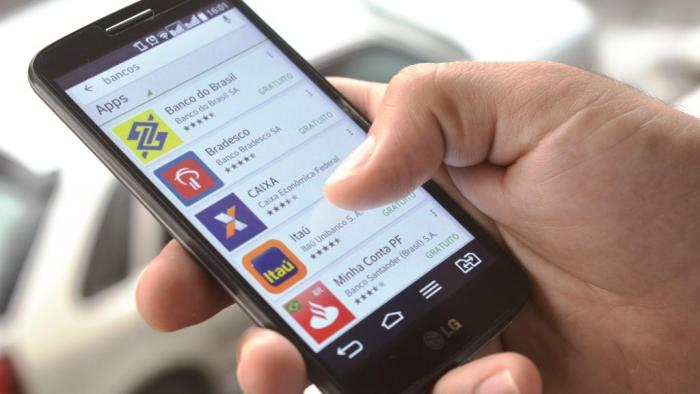
\includegraphics[width = 10cm]{Imagens/mobilebanking.jpg}
    \caption{Aplicações de banco móvel}
    \label{MobileBanking}
    \end{figure}
    
    Uma pesquisa encomendada pela Federação Brasileira de Bancos (FEBRABAN) e realizada pela empresa \citeonline{Deloitte2021} sobre tecnologia bancária revelou um aumento de 20\% no número de transações realizadas por dispositivos móveis de 2019 para 2020. Enquanto em 2019 foram efetuadas 37 bilhões de transações, no ano seguinte esse número saltou para 52,9 bilhões. Esse crescimento foi impulsionado pela pandemia e pelo programa de auxílio emergencial e essa combinação de fatores consolidou os celulares e outros dispositivos móveis como um dos principais canais de atendimento no setor bancário, como apresentado na figura \ref{febran}.
    
    \begin{figure}[H]
    \centering 
    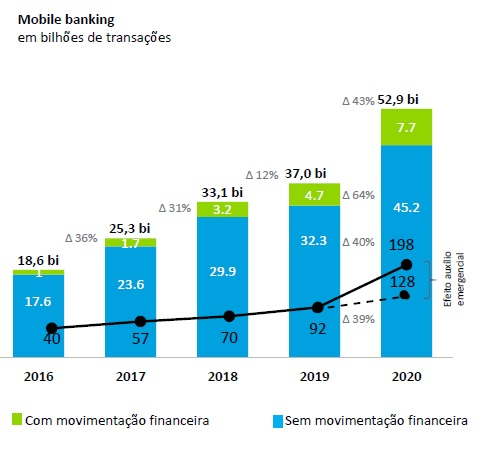
\includegraphics[width = 11cm]{Imagens/febran.jpg}
    \caption{Número de transações mobile}
    Fonte: \citeonline{Deloitte2021}
    \label{febran}
    \end{figure}
    
    
    Nesse sentido, a segurança da informação desempenha um papel fundamental no contexto das aplicações bancárias móveis. Dada a crescente popularidade destas tecnologias, é importante garantir que os dados sensíveis dos utilizadores sejam protegidos. As transações financeiras e o acesso a informações pessoais estão em risco, e as violações de segurança podem ter consequências graves, como furto financeiro, fraude e até mesmo comprometimento da identidade do usuário. Dessa forma, investir em medidas de segurança robustas não apenas tranquilizará seus clientes, mas também aumentará sua confiança ao usar esses aplicativos. 
    
    A segurança da informação não é apenas uma prioridade, mas uma necessidade para que os serviços bancários móveis continuem a evoluir e a beneficiar os consumidores de uma forma segura e eficaz. Para fazer esses aplicativos seguros é importante entender os problemas de segurança que ele traz, como por exemplo dispositivos perdidos, riscos na rede, senhas fracas, vazamentos e erros humanos. Muitas vezes, a implementação indevida ou a falta da segurança nas aplicações financeiras abre brechas para invasores. Como esse tipo de aplicativo lida diretamente com o dinheiro, eles mais do que qualquer outro devem ter a segurança impecável e lidar com esses problemas citados.
    
    Em 2015, dois pesquisadores, \citeonline{DIEGO2015}, da Universidade Estadual de Campinas (Unicamp) realizaram um estudo para identificar deficiências e fragilidades nos aplicativos de alguns bancos gigantes brasileiros para android e o resultado foi no mínimo problemático. Como mostrado na Figura \ref{PesquisaUnicamp}, foi descoberto que alguns desses aplicativos utilizavam métodos extremamente básicos de segurança e muitas vezes sabidamente vulneráveis a ataques de segurança simples, como ataques de interceptação de dados e vazamento de dados. Foram dadas notas que variam de 0 a 5 estrelas para as aplicações do topo da tabela com base na vulnerabilidade aos ataques listados na esquerda da tabela, sendo o número de estrelas diretamente proporcional qualidade da segurança da aplicação. Dessa forma, a aplicação com mais estrelas é a menos vulnerável aos ataques e a com menos estrelas é a mais vulnerável.   
    
    \begin{figure}[H]
    \centering 
    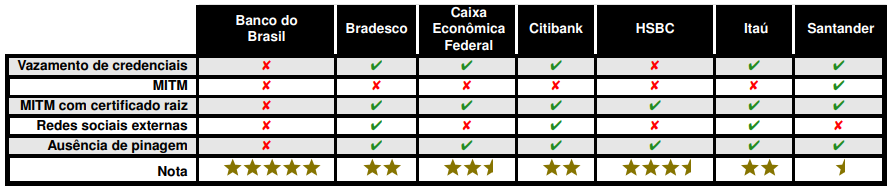
\includegraphics[width = 15cm]{Imagens/pesqunicamp.png}
    \caption{Resultado dos aplicativos Android analisados}
    \label{PesquisaUnicamp}
    Fonte: \citeonline{DIEGO2015}
    \end{figure}

    Somado a isso, como dito por \citeonline{Wang2016}, os ataques de hackers a aplicações e serviços bancários são uma ameaça crescente e significativa no mundo digital. À medida que o uso dessas tecnologias aumenta, os cibercriminosos exploram vulnerabilidades para obter acesso às informações financeiras confidenciais dos usuários e estão constantemente desenvolvendo estratégias avançadas.
    
    A todo instante são estudadas formas de desenvolver aplicações cada vez mais seguras e blindadas de ataques, identificar vulnerabilidade e propor correções antes de serem encontradas por algum indivíduo de fato malicioso. Entretanto, as aplicações bancárias incorporam características específicas, descritas por \citeonline{Islam2014}, e para garantir a segurança da informação em um cenário digital é cada vez mais complexo. 
         
    
    \section{Problemática}
    As aplicações bancárias são alvos atraentes para cibercriminosos devido à quantidade significativa de informações sensíveis que manipulam, incluindo dados pessoais, credenciais de acesso e informações financeiras. A complexidade do ecossistema móvel, combinada com práticas inadequadas de desenvolvimento e a crescente sofisticação dos ataques cibernéticos, aumenta a probabilidade de vulnerabilidades exploráveis. Tais vulnerabilidades podem resultar em ataques e outras formas de exploração que comprometem a segurança dos usuários e das instituições financeiras.
    
    A diversidade das áreas, métodos e práticas de segurança tornam difícil estabelecer diretrizes comuns e mais críticas levando em consideração as características específicas das aplicações financeiras, criando uma lacuna potencial na proteção dos dados e recursos dos usuários. 
    
    \section{Hipótese}
    A proposta de um modelo de requisitos de segurança, com base em uma revisão da literatura ressaltando ameaças e remediações eficazes, pode estabelecer diretrizes claras para o desenvolvimento seguro dessas aplicações no Android, abordando aspectos e cenários específicos do meio financeiro digital.
    
    \section{Objetivos} 
    
    O objetivo geral deste presente trabalho é propor um modelo de segurança para plataformas bancárias no Android, que seja capaz de mitigar os principais riscos e ameaças encontrados no cenário, bem como contribuir para a compreensão aprofundada e promoção da segurança da informação nessas aplicações. 
    
    Os objetivos específicos incluem:

    \begin{itemize}[topsep=3pt, partopsep=3pt, itemsep=3pt, parsep=3pt]
        \item Pesquisa: Realizar uma pesquisa de revisão visando entender, selecionar e desmistificar os principais pontos críticos de segurança em aplicações bancárias móveis e suas remediações.
        \item Criação: Propor um modelo de requisitos de segurança, com base nas informações obtidas na pesquisa anterior, que mitigue as principais ameaças encontradas.  
        \item Avaliação: Avaliar a eficácia e a viabilidade do modelo de requisitos de segurança proposto por meio de uma análise comparativa com certificações de segurança reconhecidas no mercado e de um estudo de caso. 
    \end{itemize}
    
    \section{Justificativa} 
    
    A disseminação de aplicativos bancários móveis na plataforma Android revolucionou a maneira pela qual os indivíduos conduzem transações financeiras, oferecendo maior conveniência e acessibilidade. No entanto, esse aumento na popularidade atraiu o interesse de agentes mal-intencionados, que veem essas plataformas como alvos lucrativos para possíveis ataques cibernéticos.

    A justificativa para este trabalho reside na necessidade premente de combater essas vulnerabilidades. A segurança nos aplicativos bancários é fundamental não apenas para proteger as informações confidenciais do usuário, mas também para manter a integridade e a confiabilidade da infraestrutura financeira digital. Dada a crescente dependência das tecnologias móveis, as violações de segurança têm o potencial de levar a perdas financeiras significativas e manchar a reputação das instituições envolvidas.
    
    \section{Resultados esperados} 
    Com a conclusão deste trabalho, espera-se obter um modelo de segurança para desenvolvedores de aplicações bancárias e com isso a minimização de riscos e ameaças na implementação e uso de aplicações bancárias, promovendo uma cultura de segurança mais sólida e específica.

    \section{Organização do trabalho}
    Este trabalho foi estruturado em seis capítulos, sendo eles:  
    
    No capítulo 2, "Referencial Teórico", são abordados os principais conceitos e teorias relacionados à segurança da informação, ao sistema operacional Android, às vulnerabilidades e ameaças em aplicações bancárias móveis, e à engenharia de requisitos. Este capítulo discute os conteúdos relevantes para o desenvolvimento do modelo proposto, como a revisão da literatura a fim de buscar as maiores ameaças das aplicações bancárias. 
    
    No capítulo 3, "Metodologia da Pesquisa", descreve as metodologias utilizadas para a realização da pesquisa, incluindo o levantamento e análise de dados, a elicitação e definição de requisitos de segurança utilizando casos de uso indevido, a especificação e modelagem dos requisitos com o uso de diagramas UML, e por fim são apresentados um estudo de caso e uma avaliação do modelo de segurança proposto.
    
    No capítulo 4, "Análise de Requisitos de Segurança", são detalhados os processos de elicitação, definição e especificação dos requisitos de segurança identificados, com base nos casos de uso indevido e a modelagem dos requisitos, através de diagramas UML, ilustrando a estrutura e interações dos componentes do sistema.
    
    O capítulo 5, "Estudo de caso e Avaliação do Modelo", aborda um estudo de caso do modelo de segurança proposto em um ambiente de teste, com uma análise detalhada dos casos de uso do modelo na aplicação bancária Herd Financial. Além disso, eficácia do modelo é avaliada por meio de comparações com padrões de segurança exigidos e reconhecidos no mercado.
    
    Finalmente o capítulo 6, "Conclusão",apresenta as conclusões do estudo, destacando as contribuições do trabalho, as limitações encontradas e sugestões para pesquisas futuras.

